\documentclass[tikz,border=10pt]{standalone}
\usepackage{tikz}
\usetikzlibrary{angles,quotes,calc}

\begin{document}
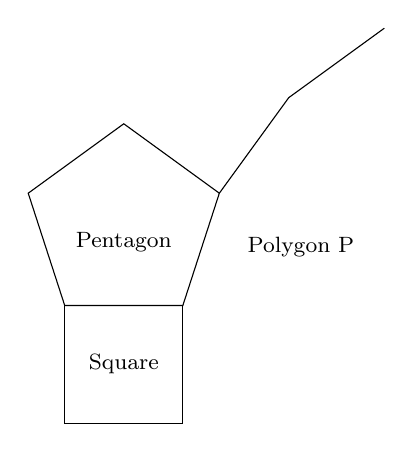
\begin{tikzpicture}[scale = 1]
    % Initial point
    \coordinate (A) at (0,0);
    % Draw pentagon
    \coordinate (A) at (0,0);
    \draw (A) -- ++(180:1.5cm) coordinate (B) -- ++(108:1.5cm) coordinate(C) -- ++(36:1.5cm) coordinate (D) -- ++(-36:1.5cm) coordinate (K) -- cycle;
    % Draw square to the bottom of the octagon
    \draw (A) -- ++(-90:1.5cm) coordinate (E) -- ++ (180:1.5cm) -- ++(90:1.5cm);

    %draw sides of larger polygon
    \draw (K) -- ++(54:1.5cm) -- ++(36:1.5cm);

    %polygon labels
    \node at (-0.75,0.8) [] {\footnotesize Pentagon};
    \node at (-0.75,-0.75) [] {\footnotesize Square};
    \node at (1.5,0.75) [] {\footnotesize Polygon P};
    
\end{tikzpicture}
\end{document}

